\documentclass[letterpaper,11pt]{scrartcl}
\usepackage[T1]{fontenc}
\usepackage[utf8]{inputenc}
\usepackage{lmodern}
\usepackage[sexy,hints]{evan}
\usepackage{hyperref}
\usepackage{graphicx}
\usepackage[english]{babel}
\usetikzlibrary{decorations.markings}
\usepackage{amsmath,unicode-math}
\usepackage{dirtytalk}
\usepackage{geometry}
 \geometry{
 left=30mm,right=25mm
 }
\usepackage{mathtools}
\usepackage{tikz}
\usetikzlibrary{calc,trees,positioning,arrows,fit,shapes,calc}
\usetikzlibrary{arrows,positioning} 
\usepackage{array}
\usepackage{wrapfig}
\usepackage{multirow}
\usepackage{tabu}
\usetikzlibrary{calc}
\usepackage{changepage}
\usepackage{caption,setspace}
\newcommand\perm[2][^n]{\prescript{#1\mkern-2.5mu}{}P_{#2}}
\newcommand\comb[2][^n]{\prescript{#1\mkern-0.5mu}{}C_{#2}}
\begin{document}
\title{Function}
\date{October 13, 2016}
\maketitle

%%fakesection Frontmatter
\begin{abstract}
	\sffamily\small
	Mathematicians just love sigma notation for two reasons.
	First, it provides a convenient way to express a long or even infinite series.
	But even more important, it looks really cool and scary,
	which frightens nonmathematicians into revering mathematicians
	and paying them more money.

	\medskip
	
	--- \emph{Calculus II for Dummies} % Mark Zegarelli
\end{abstract}
\subsection*{Acknowledgments}
\textsc{Thanks} to Zack Chroman, Michael Diao,
Steven Hao, Ryan Kim, Kevin Qian, Colin Tang, Michael Tang, Tyler Zhu,
for helpful suggestions and comments.

\tableofcontents
\eject
\section{Definition}
Function is a special case of relation, from a non empty set $A$ to a non empty set $B$, that associates each member of $A$ to a unique member of $B$. Symbolically, we write $\textit{\textbf{f}} : A \rightarrow B$. We read it as \say{$f$ is a function from $A$ to $B$}.
Set $A$ is called domain of $f$ and set $B$ is called co-domain of $f$.
For example, let $A = \{1, 0, -1\}$ and $B=\{0, 1, 2\}$. Then $A\times B = \{(1, 0), (1, 1), (1, 2), (0, 0), (0, 1), (0, 2), (-1, 0),(-1, 1), (-1, 2)\}$
Now, \say{$f: A \rightarrow B$ defined by $f(x) = x^2$} is the function such that $f = \{(1, 1), (0, 0), (-1, 1)\}$. $f$ can also be show diagramatically by following picture:

\begin{figure}[h]
 \centering
 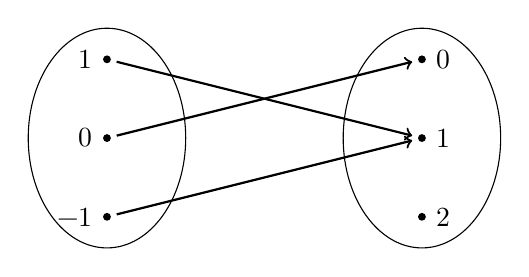
\begin{tikzpicture}[ele/.style={fill=black,circle,minimum width=.8pt,inner sep=1pt},every fit/.style={ellipse,draw,inner sep=-2pt}]
  \node[ele,label=left:$1$] (a2) at (0,3) {};    
  \node[ele,label=left:$0$] (a3) at (0,2) {};
  \node[ele,label=left:$-1$] (a4) at (0,1) {};

  \node[ele,,label=right:$0$] (b2) at (4,3) {};
  \node[ele,,label=right:$1$] (b3) at (4,2) {};
  \node[ele,,label=right:$2$] (b4) at (4,1) {};

  \node[draw,fit= (a2) (a3) (a4),minimum width=2cm] {} ;
  \node[draw,fit=  (b2) (b3) (b4),minimum width=2cm] {} ;  
  \draw[->,thick,shorten <=2pt,shorten >=2] (a2) -- (b3);
  \draw[->,thick,shorten <=2pt,shorten >=2] (a3) -- (b2);
  \draw[->,thick,shorten <=2pt,shorten >=2] (a4) -- (b3);
 \end{tikzpicture}
\end{figure}

Every function say $f : A \rightarrow B$ satisfies the following conditions:\\
(a) $f \subseteq A\times B$, (b) $\forall a\in A \Rightarrow (a, f(a)) \in f$ and (c) $(a, b)\in f\, \&\, (a, c) \in f \Rightarrow b = c$
\begin{example}
Which of the following correspondences can be called a function ?
\begin{align*}
&(a) f(x) = x^3 ;&\, &\{–1, 0, 1\} \rightarrow \{0, 1, 2, 3\}\\
&(b) f(x) = \pm \sqrt{x} ;&\, &\{0, 1, 4\} \rightarrow \{–2, –1, 0, 1, 2\}\\
&(c) f(x) = \sqrt{x} ;&\, &\{0, 1, 4\} \rightarrow \{–2, –1, 0, 1, 2\}\\
&(d) f(x) = -\sqrt{x} ;&\, &\{0, 1, 4\} \rightarrow \{–2, –1, 0, 1, 2\}
\end{align*}
\end{example}

\begin{soln}
$f(x)$ in (C) \& (D) are functions as definition of function is satisfied. while in case of (A) the given relation is not a function, as $f(-1) \not\in $ codomain. Hence definition of function is not satisfied. While in case of (B), the given relation is not a function, as $f(1) = \pm 1$ and $f(4) = \pm 2$ i.e. element 1 as well as 4 in domain is related with two elements of codomain. Hence definition of function is not satisfied
\end{soln}
\end{document}